\documentclass{article}
\usepackage{amsmath,amssymb,amsthm}
\usepackage{tikz}
\usepackage{graphicx}
\usepackage{hyperref}

\title{Nonlinear Dynamical Systems and Chaos}
\author{}
\date{}

\begin{document}
\maketitle

\section{Introduction}

Nonlinear dynamical systems are systems in which the change of the state variables is governed by nonlinear differential equations or mappings. These systems often exhibit complex behaviors, such as bifurcations, limit cycles, and chaos.

\textbf{Chaos} is defined as a deterministic yet unpredictable behavior in nonlinear systems, characterized by sensitivity to initial conditions, aperiodic long-term behavior, and fractal structures in phase space.

\section{Phase Space, Poincar\'{e} Sections, Time-Step Maps, and Fixed Points}

\subsection{Phase Space}
The phase space of a dynamical system is a multidimensional space where each dimension corresponds to one of the system's state variables. The state of the system at any given time is represented by a point in this space. 

For example, the state of a pendulum can be described by its angle $\theta$ and angular velocity $\dot{\theta}$. These variables define a two-dimensional phase space.

\subsection{Poincar\'{e} Sections}
A Poincar\'{e} section is a method to reduce the dimensionality of a continuous dynamical system by sampling the phase space at regular intervals. It provides a discrete map of the system and helps visualize periodic and chaotic behaviors. For example, in a double pendulum, a Poincar\'{e} section might sample points where one angular variable reaches zero.

\subsection{Time-Step Maps}
A time-step map samples the state of a system at fixed intervals, creating a sequence of states. This is often used to analyze the discrete evolution of systems and identify fixed points or periodic orbits.

\subsection{Fixed Points}
Fixed points are states where the system remains unchanged over time. If $\mathbf{x} = \mathbf{f}(\mathbf{x})$, then $\mathbf{x}$ is a fixed point. Stability of fixed points can be analyzed using the Jacobian matrix of $\mathbf{f}(\mathbf{x})$ at the fixed point.

\subsubsection{Example of Jacobian Matrix Analysis}
Consider a two-dimensional system governed by the equations:
\[
\dot{x} = ax + by, \quad \dot{y} = cx + dy.
\]
The Jacobian matrix $J$ at a fixed point $(x^*, y^*)$ is given by:
\[
J = \begin{bmatrix}
\frac{\partial \dot{x}}{\partial x} & \frac{\partial \dot{x}}{\partial y} \\
\frac{\partial \dot{y}}{\partial x} & \frac{\partial \dot{y}}{\partial y}
\end{bmatrix} = \begin{bmatrix}
a & b \\
c & d
\end{bmatrix}.
\]
To analyze stability, compute the eigenvalues $\lambda$ of $J$ by solving the characteristic equation:
\[
\det(J - \lambda I) = 0 \implies \lambda^2 - (a+d)\lambda + (ad - bc) = 0.
\]
The eigenvalues determine the stability:
\begin{itemize}
  \item If all eigenvalues have negative real parts, the fixed point is stable.
  \item If any eigenvalue has a positive real part, the fixed point is unstable.
  \item Complex eigenvalues with negative real parts indicate a stable spiral.
\end{itemize}

\section{Discrete Maps and the Logistic Map}

\subsection{Definition of Discrete Maps}
Discrete maps describe the evolution of a system through iterations of a function. If $x_n$ represents the state at step $n$, then the next state is given by $x_{n+1} = f_r(x_n)$, where $r$ is a control parameter.

\subsection{The Logistic Map}
The logistic map is a one-dimensional discrete map defined by:
\[
x_{n+1} = r x_n (1 - x_n),
\]
where $x_n$ is the normalized population at step $n$, and $r$ is the growth rate.

This map models population dynamics with resource competition. For example, in a rabbit population on an island, $x_n$ represents the ratio of the population to the carrying capacity.

\subsection{Effect of the Parameter $r$}
For small values of $r$, the population stabilizes at a fixed point. As $r$ increases, the system undergoes bifurcations:
\begin{itemize}
  \item $1 < r < 3$: Convergence to a single fixed point.
  \item $3 < r < 3.57$: Period-doubling bifurcations, leading to oscillations between 2, 4, 8, etc., states.
  \item $r > 3.57$: Onset of chaos, where the population fluctuates unpredictably.
\end{itemize}

\begin{figure}[h!]
\centering
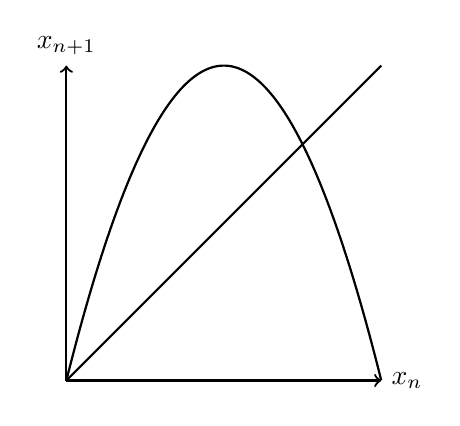
\begin{tikzpicture}
\draw[thick,->] (0,0) -- (4,0) node[right] {$x_n$};
\draw[thick,->] (0,0) -- (0,4) node[above] {$x_{n+1}$};
\draw[thick,domain=0:4,samples=100] plot (\x,{4*\x*(1-\x/4)});
\draw[thick] (0,0) -- (4,4);
\end{tikzpicture}
\caption{Cobweb diagram illustrating the logistic map.}
\end{figure}

\subsection{Bifurcations and Period Doubling}
Bifurcations occur when a small change in $r$ leads to a qualitative change in the system's behavior. Period doubling is a sequence of bifurcations where the periodicity of the system doubles with each step, eventually leading to chaos.

\subsection{Sensitivity to Initial Conditions}
Chaotic systems exhibit extreme sensitivity to initial conditions. Two nearly identical initial states diverge exponentially over time, making long-term predictions impossible.

\subsection{Power Spectrum}
The power spectrum of a chaotic system is broad and continuous, unlike the discrete peaks of a periodic system. This reflects the aperiodic nature of chaos.

\section{Fractal Patterns and Cobweb Graphs}

\subsection{Fractal Patterns}
Chaotic systems often exhibit fractal structures in their phase space. These structures have self-similarity and fractional dimensions, providing insight into the system's complexity.

\subsection{Cobweb Graphs}
A cobweb graph visualizes iterations of a discrete map. Starting from an initial point, a trajectory is plotted using vertical and horizontal lines between the map's function and the diagonal $x_{n+1} = x_n$. This technique highlights fixed points and periodic orbits.

\section{Conclusion}
Nonlinear dynamical systems and chaos provide a framework for understanding complex, unpredictable behaviors in natural and engineered systems. Tools like phase space, bifurcation analysis, and fractal geometry are essential for analyzing such phenomena.

\end{document}
